% Chapter 2

\chapter{Theoretical Discussion}\label{chap:Theory}
What follows is a review of the theory for arbitrarily high order finite elements for Lagrangian hydrodynamics. Much of this formulation previously appeared in \cite{DobrevEllisKolevRieben2010}.

\section{Euler Equations in a Lagrangian Frame}
The Navier-Stokes equations can be simplified for high Reynolds number flows by assuming that inertial forces are much more significant than viscous forces. Thus all viscous terms can be neglected. This simplified set of four equations are known as the Euler equations and must be solved for four unknowns: velocity $\vec{v}$, density $\rho$, internal energy $e$, and pressure $p$. The Euler equations in a Lagrangian frame are listed below, where $\frac{\mathrm{d}}{\mathrm{d}t}$ represents the total (or advective) derivative. Also please note that these equations are valid for gas dynamics, not the more general case of solid dynamics where scalar pressures would need to be replaced by stress tensors.
\begin{eqnarray}
  \text{Momentum Conservation:}\;\;\;\;\;\; 
  \rho \frac{\mathrm{d} \vec v}{\mathrm{d} t}        &=& 
  - \Grad p                                            
  \label{eq:MomentumConservation}                     \\
  \text{Mass Conservation:}\;\;\;\;\; 
  \frac{1}{\rho}\frac{\mathrm{d} \rho}{\mathrm{d} t} &=& 
  - \Div \vec v                                          
  \label{eq:MassConservation}                         \\
  \text{Energy Conservation:}\;\;\;\;\;\; 
  \rho \frac{\mathrm{d} e}{\mathrm{d} t}             &=& 
  - p \Div \vec v                                                            
  \label{eq:EnergyConservation}                       \\
  \text{Equation of State:}\;\;\;\;\;\;\;\;\;\;\; 
  p                                              &=& 
  EOS(\rho,\; e)                                                          
  \label{eq:EquationOfState}                        
\end{eqnarray}
The Euler equations describe the relationship between fluid motion and the kinematic properties of the fluid such as pressure, energy, and density over a spatial domain $\Omega$. The Equation of State (EOS) describes the relationship between the thermodynamic state variables and provides the necessary closure to the set of equations. In a hydrocode the density and energy of a material are fairly straightforward to calculate each time step. The EOS takes these variables as inputs and allows us to calculate the pressure of the material which is necessary for predicting the future movement of the fluid. The total mass in the spatial domain $\Omega$ is defined to be
\newEq{Mass}{
  m \equiv \int_{\Omega} \rho    
}
Furthermore, the total kinetic energy in the spatial domain 
$\Omega$ is defined as
\newEq{KEDef}{
  KE = \frac{1}{2} \int_{\Omega} {\rho \vec v} \cdot \vec v    
}
The total internal energy in the spatial domain $\Omega$ is defined
as
\newEq{IEDef}{
  IE = \int_{\Omega} \rho e
}
The total energy contained in the spatial domain $\Omega$ is thus
\newEq{TOTEDef}{
  E = KE + IE 
}
If the spatial domain $\Omega$ contains no energy sources (or sinks)
and there is no flux of energy and/or mass out of the boundary of the
domain, $\partial \Omega$, then the total energy contained in 
$\Omega$ is a constant for all time
\newEq{ECons}{
  \frac{\mathrm{d} E}{\mathrm{d} t} = 0
}

\section{A Brief Summary of the Finite Element Method}
The finite element method (FEM) is a powerful numerical technique for solving partial differential equations (PDE) on complicated domains. In contrast to the finite difference method which finds a solution to a finite difference approximation of the differential equation, the FEM finds an approximate solution to the weak form of the original differential equation restricted to a (finite element) subspace. 

\subsection{The Weak Statement of the Problem}\label{sec:WeakStatement}
The first step in the solution to any problem is to first define the problem itself. The FEM requires that the problem be described in a specific format known as the variational or weak statement of the problem \cite{Hughes1987}. Any differential equation can be reformulated to fit into this required format. In brief, you must multiply the differential equation by test function and integrate both sides of the resulting equation over the problem domain. After an integration by parts some of the derivatives are transferred over to the test functions. The resulting system of equations is the variational formulation of the problem. For our purposes, the test functions are chosen to be the same set as the basis functions according to Galerkin's method. We formulate the weak statement of the Euler equations in \refSec{MomentumCons}.

\subsection{Basis Functions}
The approximation to the solution of the differential equation is built up from a set of analyst-selected \emph{basis functions}. The solution to the PDE is assumed to be the summation of all basis functions multiplied with a set of unknown coefficients known as degrees of freedom (DOF). Generally, the basis functions may be any function at all, but typically they are chosen to be piecewise continuous polynomials defined such that they are valued 1 at their own DOF and zero at all others. Thus, when all basis functions are summed up with their respective DOF coefficients, the overall solution will assume values of a DOF at that DOF location and interpolate polynomially to adjacent DOFs. 

As mentioned previously, traditionally staggered grid approaches have associated velocities with vertices and thermodynamic variables have been associated with zone centers and defined as piece-wise constant values. Our general FEM approach treats each field -  $\vec{v}$, $\rho$, $e$, and $p$ as finite element functions on the computational mesh $\tilde\Omega(t)$ with the following expansions
%  for $\vec{x}\in\Omega(t)$

\begin{eqnarray}
  \vec v(\vec x,t) \approx
  \sum_{i}^{N_\mathbf{v}} \mathbf{v}_i(t) \; \vec w_i(\vec x, t) \,,
  \label{eq:DiscreteV} \\
  \rho(\vec x,t)  \approx
  \sum_{i}^{N_\mathbf{r}} \mathbf{r}_i(t) \; \psi_i(\vec x, t) \,, \label{eq:DiscreteRho} \\
  e(\vec x,t)  \approx
  \sum_{i}^{N_\mathbf{e}} \mathbf{e}_i(t) \; \theta_i(\vec x, t) \,, \label{eq:DiscreteE} \\
  p(\vec x,t) \approx
  \sum_{i}^{N_\mathbf{p}} \mathbf{p}_i(t) \; \phi_i(\vec x, t) \,.
  \label{eq:DiscreteP}
\end{eqnarray}

These basis functions will move with the mesh. Furthermore, for simplicity and ease of computation basis functions will be defined on the reference zone and mapped to physical space via the Jacobian of transformation, see \ref{sec:JacobianTransformation}.

\begin{figure}[h!]
 \centering
   \centerline{
    \mbox{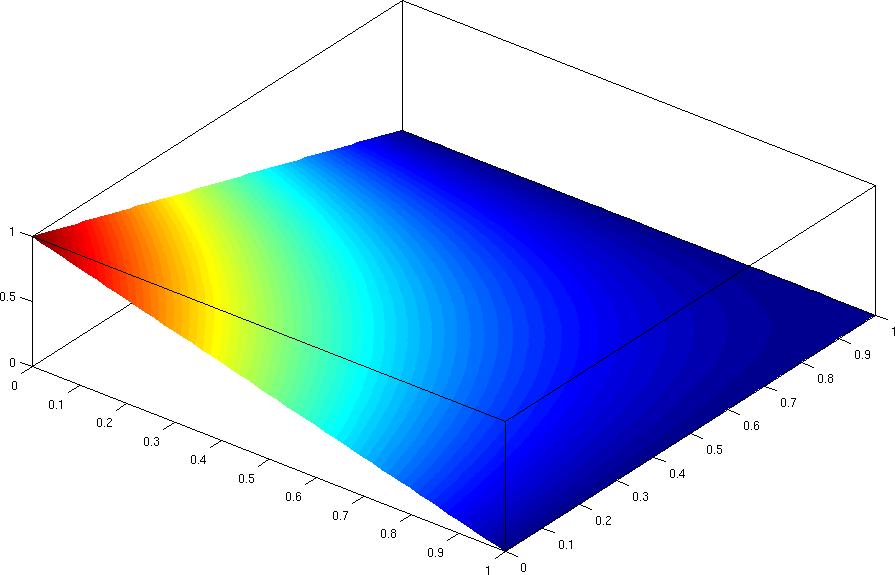
\includegraphics[width=2.00in]{./Figures/Q1Basis.png}}
    \mbox{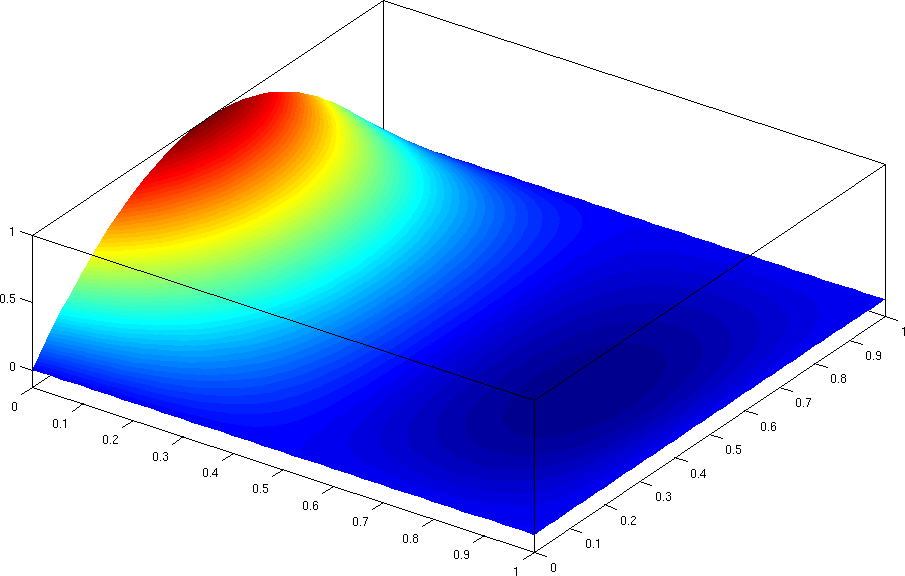
\includegraphics[width=2.00in]{./Figures/Q2Basis.png}}
    \mbox{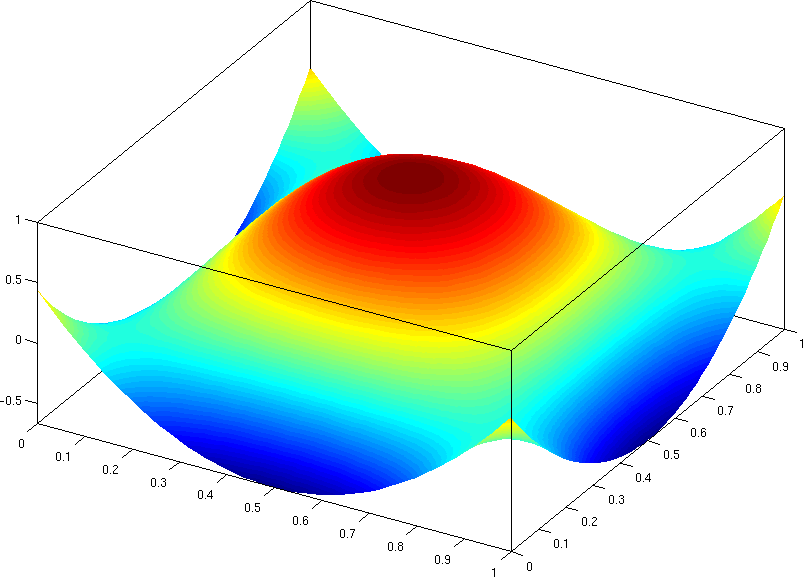
\includegraphics[width=2.00in]{./Figures/Q2dBasis.png}}
  }
 \caption{Examples of 2D basis functions on a reference zone: a standard $Q_1$ bi-linear function that interpolates at nodes \textit{(left)}, a $Q_2$ bi-quadratic function defined at the Gauss-Lobatto quadrature points \textit{(center)} and a $Q_2$ bi-quadratic function defined at the Gauss-Legendre quadrature points \textit{(right)}.}
 \label{fig:ExBasis}
\end{figure}

\section{Mesh}
The basic premise of the Finite Element Method (FEM) is to divide a large complicated problem into a system of smaller simpler problems. In order to do this, we need to divide the problem domain into a number of non-overlapping volumes or zones (aka elements). The governing equations are then solved on each of these smaller domains and assembled to obtain an overall solution to the problem. 

\subsection{Domain Decomposition}
The FEM requires us to take many integrals as we set up the system of simple problems. It is difficult to take an integral over an arbitrary region, especially in an automated fashion. Thus, the first step is to divide the arbitrarily complicated problem domain into a number of simpler zones. In 2-D These zones or elements are usually three- or four-sided but can be more complicated. Each side is defined by a polynomial curve. Traditionally, first order curves, i.e. straight lines are used to connect vertices, but quadratic, cubic, or even higher order curves can be used. \refFig{DomainDecomp} illustrates this process.

\begin{figure}[h!]
\begin{center}
$\begin{array}{c@{\hspace{.35in}}c@{\hspace{.35in}}c}
\includegraphics*[height=2.0in,keepaspectratio=true]{./Figures/DomDecomp1.png}  &  
\raisebox{0.75in}{{\Huge $\mathbf \longrightarrow$}} &
\includegraphics*[height=2.0in,keepaspectratio=true]{./Figures/DomDecomp2.png}   \\
\mbox{\Large $\mathbf{\Omega}(t_0)$} & & \mbox{\Large{$\tilde{\mathbf{\Omega}}(t_0)\equiv \bigcup_z \mathbf{\Omega}_z(t_0)$}} \\
\end{array}$
\end{center}
\caption{Domain decomposition for a finite element mesh}
\label{fig:DomainDecomp}
\end{figure}

Now that we have divided our problem domain into a number of smaller zones, we can link these together to form the \emph{computational mesh}, denoted by $\tilde{\Omega}$ and defined as
\newEq{FEMMesh}{
  \Omega(t_0) \approx \tilde{\Omega}(t_0) \equiv \bigcup_z \Omega_z (t_0)
}
The computational mesh is composed of two sets of information. The \emph{topology}\label{sec:topology} defines the connectivity of the mesh: which nodes belong to which element and which elements share faces, etc. The \emph{geometry} connects nodes to coordinates in physical space. For example, if you wish to compute the volume of element $n$, you must first follow the topology to determine which nodes are connected to element $n$ and the ordering of these nodes. Then you must follow the geometry to find the physical coordinates of these nodes. Once you know the physical locations and ordering of the nodes, then you can perform the desired calculations. 

Curved physical geometries occur frequently in problems of engineering interest. The Sedov explosion problem is a simplified model of an explosive blast propagating through a gas, a problem significant to many fields of engineering. If we take an initially straight Cartesian mesh and continuously apply the exact solution of the Sedov explosion problem to the nodes and edges, we obtain the mesh shown in \refFig{ExactSedovMesh}. The obviously curved elements, especially surrounding the origin motivate the need for zones with curved edges. We would eliminate much of the domain decomposition error if elements had the flexibility to follow curved geometries more closely.

\begin{figure}[h!]
 \centering
 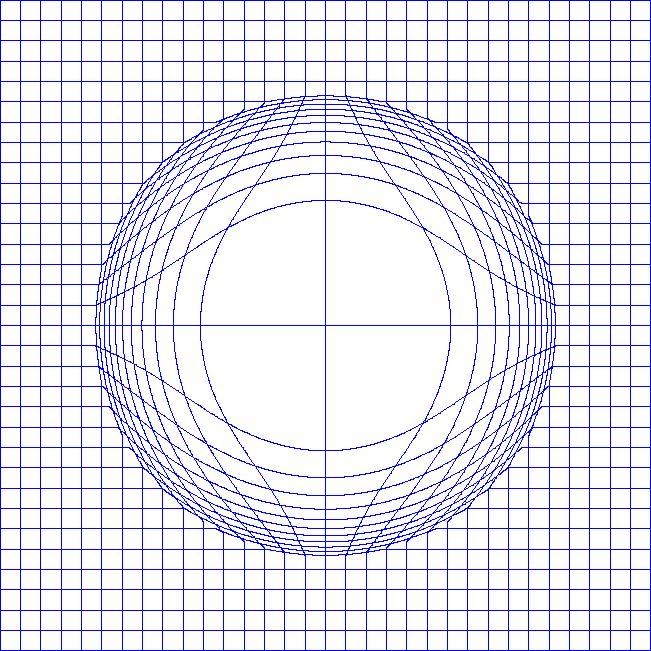
\includegraphics[width=5in,keepaspectratio=true]{./Figures/sedovCart.png}
 % sedovCart.png: 683x683 pixel, 72dpi, 24.09x24.09 cm, bb=0 0 683 683
 \caption{An initial Cartesian mesh is continuously deformed according to the exact solution of the Sedov blast wave.}
 \label{fig:ExactSedovMesh}
\end{figure}

\subsection{Mesh Motion}
By the definition of the Lagrangian framework, for all interesting flows, the computational mesh will move during the process of the simulation. Each element can be thought of as a small volume of fluid that will move and distort in reaction to pressure fields acting on it. We move each volume by tracking a finite number of particles on the boundaries of (and possibly within) that volume known as the \emph{position degrees of freedom}. During each time step, each position degree of freedom is moved according its corresponding velocity degree of freedom and the mesh is reconstructed for the next time step, as illustrated by \refFig{MeshMotion}.

\begin{figure}[h!]
 \centering
   \centerline{
    \mbox{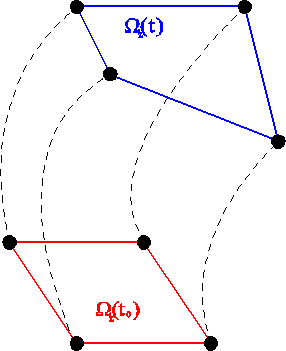
\includegraphics[width=2.00in]{./Figures/motion1.png}}
    \mbox{\hspace*{0.5in}}
    \mbox{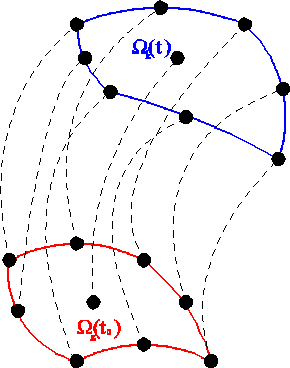
\includegraphics[width=2.00in]{./Figures/motion2.png}}
  }
 % sedovCart.png: 683x683 pixel, 72dpi, 24.09x24.09 cm, bb=0 0 683 683
 \caption{A zone $\Omega_z(t)$ is reconstructed from the evolution of only a few of its points (particles) indicated by black dots. Shown are two specific choices corresponding to the traditional $Q_1$ zone (left) and a high order $Q_2$ zone with curvilinear boundaries (right).}
 \label{fig:MeshMotion}
\end{figure}

\subsection{Jacobian of Transformation}\label{sec:JacobianTransformation}
Even an initially perfectly Cartesian mesh can get rather distorted in the process of a simulation. As mentioned previously, one of the motivations to divide the problem domain into regular zones with regular topology was to ease the process of integration. But integrating over arbitrary distorted zones, especially autonomously, is not a completely trivial matter. This is where the Jacobian of transformation comes in. 

The Jacobian matrix is used as a mapping from a standard reference zone $\tilde{\Omega_z} = [0,1]^2$ to physical space, see \refFig{JacMapping}. We can write the mapping in a functional form as 

\begin{equation}
 \vec{x}=\Phi(\hat{\vec{x}},t), \label{eq:parametricMapping}
\end{equation} 

where $\vec{x}$ denotes a point in physical space and $\hat{\vec{x}}$ denotes the corresponding point in the reference zone. This coordinate transformation is referred to as the parametric mapping and is defined by the physical coordinates of the particles associated with each zone. For the case of a traditional $Q_1$ zone geometry consisting of four vertices connected by straight lines, the parametric mapping is bilinear. This thesis explores some of the befits of high order mappings such as $Q_2$ (bi-quadratic) which produce zones with curvilinear geometry as shown in \refFig{JacMapping}. These parametric mappings are computed for each zone using an interpolating polynomial expansion of the form 

\begin{equation}
 \Phi_z(\hat{\vec{x}},t)=\sum_i \vec{x}_{z,i}(t) \eta_i(\hat{\vec{x}}),
\end{equation}

where $\vec{x}_{z,i}(t)$ denote the physical coordinates of the particles describing the zone $z$ at time $t$, see \refFig{MeshMotion}, and $\eta_i$ is the (high order) nodal basis function associated with particle $i$. The collection of all particle coordinates listed consecutively in a vector array is denoted by $\mathbf{x}(t)$. We define the Jacobian matrix for this mapping as

\begin{equation}
 \mathbf{J}_z=\vec{\nabla}_{\hat{\vec{x}}} \Phi_z \quad\quad \mathrm{or} \quad\quad \left(\mathbf{J}_z\right)_{i,j}=\frac{\partial x_i}{\partial \hat{x}_j} \mathrm{.}
\end{equation}

Note that in general, the Jacobian matrix is a \emph{function} of the reference coordinates $\hat{\vec{x}}$ and therefore varies in a zone. 

For bi-linear elements, the Jacobian is defined according to \refEq{Q1Jacobian}, while bi-quadratic elements use the much more complicated entries in \refEq{Q2Jacobian} to assemble the Jacobian matrix. %Bear in mind that these example Jacobian matrices are for 2-D elements, their 3-D equivalent would be 3$\times$3 matrices. %For the full details of a 

\begin{eqnarray}\label{eq:Q1Jacobian}
\mathbf{J}_z(\hat x,\hat y)=\left[
\begin{array}{cc}
 x_2 - x_1 + \hat y(x_1 + x_3 - x_2 - x_4) & x_4 - x_1 + \hat x(x_1 + x_3 - x_2 - x_4) \\
 y_2 - y_1 + \hat y(y_1 + y_3 - y_2 - y_4) & y_4 - y_1 + \hat x(y_1 + y_3 - y_2 - y_4)
\end{array} \right] \nonumber \\
\end{eqnarray}

\begin{figure}[htbp]
\centering
  \includegraphics*[height=2.0in,keepaspectratio=true]{./Figures/Q2_Element_Ref.png}
  \hspace{8mm}
  \raisebox{0.95in}{{\Huge $\mathbf \longmapsto$}}
  \hspace{8mm}
  \includegraphics*[height=2.0in,keepaspectratio=true]{./Figures/Q2_Element_Phys.png}
  \caption{Example of a $Q_2$ bi-quadratic mapping from a reference zone
          (\emph{left}) to a Lagrangian zone (\emph{right}) defined by
          the locations of the 9 Lagrangian particles
          (black dots).
  \label{fig:JacMapping}}
\end{figure}

\clearpage
\begin{eqnarray}\label{eq:Q2Jacobian}
   J_{1,1}  & = &
         (\hat y - 1)(2\hat y - 1)(4\hat x - 3)x_1  
       + (\hat y- 1)(2\hat y - 1)(4\hat x - 1)x_2 \nonumber \\
   & & + \hat y(2\hat y - 1)(4\hat x - 1)x_3  
       + \hat y(2\hat y- 1)(4\hat x - 3)x_4 \nonumber \\
   & & - 4(\hat y - 1)(2\hat y - 1)(2\hat x - 1)x_5 
       - 4\hat y(\hat y - 1)(4\hat x - 1)x_6 \nonumber \\
   & & - 4\hat y(2\hat y - 1)(2\hat x - 1)x_7 
       - 4\hat y(\hat y - 1)(4\hat x- 3)x_8 \nonumber \\
   & & + 16\hat y(\hat y - 1)(2\hat x - 1)x_9 \nonumber \\
%
   J_{1,2} & = &
         (4\hat y - 3)(\hat x - 1)(2\hat x - 1)x_1 
       + \hat x(4\hat y - 3)(2\hat x - 1)x_2 \nonumber \\
   & & + \hat x(4\hat y - 1)(2\hat x - 1)x_3 
       + (4\hat y - 1)(\hat x - 1)(2\hat x - 1)x_4 \nonumber \\
   & & - 4\hat x(4\hat y - 3)(\hat x -1)x_5 
       - 4\hat x(2\hat y -1)(2\hat x - 1)x_6 \nonumber \\
   & & - 4\hat x(4\hat y - 1)(\hat x - 1)x_7 
       - 4(2\hat y - 1)(\hat x - 1)(2\hat x - 1)x_8 \nonumber \\
   & & + 16\hat x(2\hat y - 1)(\hat x - 1)x_9 \nonumber \\
%
   J_{2,1} & = &
         (\hat y - 1)(2\hat y - 1)(4\hat x - 3)y_1  
       + (\hat y- 1)(2\hat y - 1)(4\hat x - 1)y_2 \nonumber \\
   & & + \hat y(2\hat y - 1)(4\hat x - 1)y_3  
       + \hat y(2\hat y- 1)(4\hat x - 3)y_4 \nonumber \\
   & & - 4(\hat y - 1)(2\hat y - 1)(2\hat x - 1)y_5 
       - 4\hat y(\hat y - 1)(4\hat x - 1)y_6 \nonumber \\
   & & - 4\hat y(2\hat y - 1)(2\hat x - 1)y_7 
       - 4\hat y(\hat y - 1)(4\hat x- 3)y_8 \nonumber \\
   & & + 16\hat y(\hat y - 1)(2\hat x - 1)y_9 \nonumber \\
%
   J_{2,2} & = &
         (4\hat y - 3)(\hat x - 1)(2\hat x - 1)y_1 
       + \hat x(4\hat y - 3)(2\hat x - 1)y_2 \nonumber \\
   & & + \hat x(4\hat y - 1)(2\hat x - 1)y_3 
       + (4\hat y - 1)(\hat x - 1)(2\hat x - 1)y_4 \nonumber \\
   & & - 4\hat x(4\hat y - 3)(\hat x -1)y_5 
       - 4\hat x(2\hat y -1)(2\hat x - 1)y_6 \nonumber \\
   & & - 4\hat x(4\hat y - 1)(\hat x - 1)y_7 
       - 4(2\hat y - 1)(\hat x - 1)(2\hat x - 1)y_8 \nonumber \\
   & & + 16\hat x(2\hat y - 1)(\hat x - 1)y_9 \nonumber \\
\end{eqnarray}

\section{Semi-Discrete FEM Approximation}
In the semi-discrete formulation the problem has been discretized in space, but a specific time discretization has not been selected yet. Time could be discretized in a forward Euler-like scheme, a leap-frog scheme, predictor-corrector, or any other time discretization.

\subsection{Momentum Conservation}\label{sec:MomentumCons}
In order to derive a semi-discrete momentum conservation law, we start with the variational formulation or the weak statement of the problem. Multiply \refEq{MomentumConservation} by a vector valued test function $\vec w'$ and integrate over the spatial domain $\Omega(t)$:

\newEq{MomentumIntegral}{
\int\limits_{\Omega(t)}\left(\rho\frac{\mathrm{d}\vec{v}}{\mathrm{d}t}\right)\cdot \vec w'= -\int\limits_{\Omega(t)}\left(\vec{\nabla}p\right)\cdot \vec w'
}

Now, approximating the spatial domain $\Omega(t)$ with the computational mesh $\tilde \Omega(t)$, integrate the right hand side of \refEq{MomentumIntegral} and apply the divergence theorem:

\newEq{WeakMomentum}{
\int\limits_{\tilde{\Omega}(t)}\left(\rho\frac{\mathrm{d}\vec{v}}{\mathrm{d}t}\right)\cdot \vec w'
= \int\limits_{\tilde{\Omega}(t)}p\left(\vec{\nabla}\cdot\vec w'\right)
- \int\limits_{\partial\tilde{\Omega}(t)}p(\vec w'\cdot\hat{n})
}

where $\hat{n}$ is the outward pointing unit normal vector of the surface $\partial\tilde{\Omega}(t)$.

If we substitute the basis function expansions from (\ref{eq:DiscreteV}) for $\vec{v}$ and (\ref{eq:DiscreteP}) for $p$, and for code simplicity's sake assume boundary conditions that will cause the boundary integral term to vanish (otherwise we would need integrate these boundary terms and apply them as sources to the resulting equation), we arrive at
\newEq{MomentumVar3}{
  \int_{\tilde \Omega (t)}
  (\rho  \sum_i^{N_\mathbf{v}}  \frac{\mathrm{d} \mathbf{v}_i}{\mathrm{d} t} \vec w_i) \cdot \vec w' =
  \int_{\tilde \Omega (t)}
  \sum_i^{N_\mathbf{p}} \; \mathbf{p}_i \phi_i
  (\Div \vec w')  \,.
}
As mentioned in Section \refSec{WeakStatement}, we can apply Galerkin's method and pick the velocity basis functions $\vec{w}_j$ as our test functions $\vec w'$. If we do this we will arrive at the following system of linear ordinary differential equations
\newEq{MomentumVar4}{
  \sum_i^{N_\mathbf{v}}
  \frac{\mathrm{d} \mathbf{v}_i}{\mathrm{d} t}
  \int_{\tilde \Omega (t)}
  \rho (\vec w_i \cdot \vec w_j) =
  \sum_i^{N_\mathbf{p}} \mathbf{p}_i
  \int_{\tilde \Omega (t)}
  \phi_i (\Div \vec w_j)  \,.
}
In matrix form this can be written,
\newEq{GlobalMomentum}{
\boxed{
  \mathbf{M} \frac{\mathrm{d} \mathbf{v} }{\mathrm{d}t }  =
  \mathbf{D}^T \mathbf{p}
}}
where $\mathbf{M}$, $\mathbf{D}$, $\mathbf{v}$, and $\mathbf{p}$ are global matrices or vectors (arrays) that are assembled over the entire computational mesh $\tilde\Omega(t)$ with contributions from DOFs in each individual zone $z$. This is known as the assembly operation and can be written as
\begin{eqnarray*}
  \mathbf{M} = Assemble(\mathbf{M}_z), && \mathbf{D} = Assemble(\mathbf{D}_z), \\
  \mathbf{v} = Assemble(\mathbf{v}_z), && \mathbf{p} = Assemble(\mathbf{p}_z) \,.
\end{eqnarray*}
During this global assembly process the topological (see \ref{sec:topology}) information is used to sum to each degree of freedom information from all zones that it is part of. This is analogous to the idea of ``nodal accumulation'' that is present in traditional SGH codes. Note that the resulting mass matrix $\mathbf{M}$ is global in scope and, in general, requires a full linear solve \label{sec:FullLinearSolve} at each time step to arrive at the desired accelerations. This may sound computationally daunting, but some simplifications can be made to significantly speed up this process such as mass lumping. Mass lumping sums each row of the matrix to it's diagonal, reducing the accuracy while eliminating a full linear solve. In general the mass matrix is very sparse and is has not been a major computational bottleneck in the test problems considered. 

The global mass matrix must be assembled from local mass matrices $\mathbf{M}_z$ calculated for each zone. The local mass matrix can be calculated over a zone $z$
\newEq{MassMat}{
  (\mathbf{M}_z)_{i,j} \equiv  \int_{\Omega_z(t)} \rho (\vec w_i \cdot \vec w_j) \,.
}
By its construction, the mass matrix is symmetric positive definite with dimension $ndof_v \times ndof_v$ where $ndof_v$ is the number of x- or y- velocity degrees of freedom per zone. In theory, $\mathbf{M}_z$ should be $(2 \cdot ndof_v) \times (2 \cdot ndof_v)$ to account for both x- and y- velocity degrees of freedom, but in practice they are identical and a single $ndof_v \times ndof_v$ matrix can be used. For example, a $Q_1$ element has 4 x- and 4 y- velocity degrees of freedom while a $Q_2$ element has 9 x- and 9 y- velocity degrees of freedom. Thus the local mass matrix for a $Q_2$ element would be a $9 \times 9$ matrix. 
The local derivative matrix for zone $z$ is defined as
\newEq{DivMat}{
  (\mathbf{D}_z)_{i,j} \equiv \int_{\Omega_z (t)} \phi_i (\Div \vec w_j) \,.
}
The derivative matrix is a \emph{rectangular} of dimension $ndof_p \times ndof_v$ and acts as a map between the two discrete representations of velocity and pressure. It is a discrete version of the $Div$ operator. The transpose of the derivative matrix is also a discrete version of the $Grad$ operator as seen in (\ref{eq:GlobalMomentum}).

\subsection{Computing FEM Matrices}
As mentioned previously, numerical integration is at the heart of the finite element method. The mass and derivative matrices mentioned above take the brunt of this numerical integration effort. In practice, we compute these integrals by transforming them from each Lagrangian zone $\Omega_z(t)$ to the reference zone $\hat{\Omega}$ through the parametric mapping of (\ref{eq:parametricMapping}). For a general integral over a given Lagrangian zone, this transformation gives
\begin{displaymath}
  \int_{\Omega_z (t)} f = \int_{\hat \Omega _z} (f \circ \Phi) \; |\det \mathbf{J}_z|,
\end{displaymath}
for some integrand f, where ``$\circ$'' denotes composition. Integrals are approximated using quadrature of a user-selected order. This integral over the the Lagrangian zone can therefore be replaced with the following weighted sum
\newEq{ApproxIntegral}{
 \int_{\Omega_z (t)} f
%%  \int_{\hat \Omega _z} (f \circ \Phi) \; |\det \mathbf{J}_z|
 \approx
 \sum_{n=1}^{N_q}
 \alpha_n\;
 \left\{
 (f \circ \Phi) \; |\det \mathbf{J}_z|
 \right\}_{\hat{\vec x} = \hat{\vec q}_n} \,,
}
where $\alpha_n$ are the $N_q$ quadrature weights and $\hat{\vec q}_n$ are
quadrature points inside of the reference zone where the integrand is sampled
at. It is important to realize that depending on the functional form of the integrand and the order of the quadrature rule, numerical quadrature is not always exact. Thus, we have introduced additional, though reasonable, approximation error to the solution of the governing equations. Practically, Gauss-Legendre quadrature is preferred for quadrature on quadrilaterals due to great accuracy for relatively few sample points. 

\subsection{Mass Conservation} \label{sec:densityupdateeq}
By the very nature of the Lagrangian description of fluid dynamics, there is no flux across zone boundaries. Hence, the total amount of mass in a zone is constant for all time. 
\newEq{ZoneMassCons}{
  \frac{\mathrm{d} }{\mathrm{d}t} \int_{\Omega _z(t)} \rho = 0\,.
}
In order to allow for high order density field representations, we need to define high order ``mass moments'' for a given zone using the density basis functions from \refEq{DiscreteRho}:
\newEq{MassMoments}{
 \mathbf{m}_{z,i} \equiv
 \int_{\Omega _z(t)} \rho \psi_i \,.
}
We generalize the case of zonal mass conservation to the high order
mass moments by postulating that
\newEq{MassMomentConst}{
  \frac{\mathrm{d} \mathbf{m}_{z,i} }{\mathrm{d}t} = 0 \,.
}
This choice is motivated by the fact that the same equation holds in the
continuous case. Furthermore, \refEq{MassMomentConst} has the same number of
conditions as the number of unknown densities and in particular it implies
\refEq{ZoneMassCons}.
Note that for the case of a piece-wise constant density approximation
(a single mass moment), we recover the traditional definition of
zonal mass conservation. From our basis function representation of the density field \refEq{DiscreteRho}, it follows that
$$
  \mathbf{m}_{z,i}=\sum_j \mathbf{r}_{z,j}\int_{\Omega_z(t)}\psi_i\psi_j \, .
$$
Written in matrix form, we have 
$$
  \mathbf{m}_z = \mathbf{M}^{\rho}_z \mathbf{r}_z
  \qquad\text{where}\qquad
  (\mathbf{M}^{\rho}_z)_{i,j} \equiv \int_{\Omega _z(t)} \psi_i \psi_j \,.
$$
This yields the semi-discrete mass conservation law
\newEq{SemiDiscreteMass}{
\boxed{
  \frac{\mathrm{d} }{\mathrm{d}t}( \mathbf{M}^{\rho}_z \mathbf{r}_z ) = 0
}
}
The above can be viewed as a generalization of the "sub-zonal mass" concept
introduced in  \cite{CaramanaBurtonShashkov98}; it is a statement that
no mass enters or leaves a given sub-volume of the zone.
If we take the limiting case of this idea and impose mass conservation of the
form
$$
  \frac{\mathrm{d} }{\mathrm{d}t} \int_{\Omega'(t)} \rho = 0 \qquad \mbox {for any} \qquad
\Omega'(t) \subseteq \Omega_z(t) \,,
$$
then we obtain the \emph{strong mass conservation principle}\label{sec:strongmass}
\newEq{StrongMassCons}{
  \rho(t) |\det \mathbf{J}_z(t)| = \rho(t_0) |\det \mathbf{J}_z(t_0)|
}
which is a statement of mass conservation for any point in space (not just in
a variational sense). Note that the density defined by this equation is not
polynomial.

We can write the following relation between the finite element density
function defined by \refEq{SemiDiscreteMass} and the function defined by
\refEq{StrongMassCons} (denoted here by $\rho_h$ and $\rho_s$, respectively)
\newEq{DensityRelation}{
\int_{\Omega_z(t)} \rho_{h} \psi_i = \int_{\Omega_z(t)} \rho_{s} \psi_i
}
which tells us that $\rho_h$ is the projection of $\rho_s$ on the space
spanned by $\{\psi_i\}$.

\subsection{Energy Conservation}
What follows is a general derivation of energy conservation for arbitrarily high order representation. High order energy is still in the experimental stages in \texttt{Fermium}, and all numerical results are presented with piece-wise constant energies. Thus in practice, we use only \refEq{SemiDiscreteEnergyConst}.

If we multiply the energy equation, \refEq{DiscreteE} by a vector valued test function, $\theta_j$ and integrate over a local spatial domain, $\Omega_z(t)$ we arrive at a local formulation for the energy conservation equation
$$
  \int_{\Omega _z(t)} \rho \frac{\mathrm{d} e}{\mathrm{d}t} \theta_j =
  \int_{\Omega _z(t)} p (\Div \vec v) \theta_j\,.
$$
Inserting the basis function expansions for internal energy, pressure and velocity from (\ref{eq:DiscreteV} - \ref{eq:DiscreteP}) we obtain 
\newEq{SemiDiscreteEnergy}{
\boxed{
\mathbf{M}^e_z \frac{\mathrm{d} \mathbf{e}_z}{\mathrm{d}t} =
  - \mathbf{p}_z \cdot \mathbf{D}^e_{z} \cdot \mathbf{v}_z
}
}
where
$$
  (\mathbf{M}^e_z)_{i,j}     \equiv \int_{\Omega _z(t)} \rho \theta_i \theta_j
  \qquad\mbox{and}\qquad
  (\mathbf{D}^e_{z})_{i,j,k} \equiv \int_{\Omega _z(t)} \phi_i \theta_j (\Div \vec w_k) \,.
$$
Here $\mathbf{D}^e_{z}$ is tensor of rank 3 satisfying
$\mathbf{D}_{z} = \mathbf{D}^e_{z} \cdot \mathbf{1}^e_z$, i.e.,
$(\mathbf{D}_{z})_{i,k} = \sum_j (\mathbf{D}^e_{z})_{i,j,k} (\mathbf{1}^e_z)_j$,
where $\mathbf{1}^e_z$ is the zonal representation of the constant $1$ in the
internal energy space (a vector of ones for nodal finite elements).  In this
formulation, the matrix $\mathbf{F}_z = \mathbf{p}_z \cdot \mathbf{D}^e_{z}$ can
be used to generalize the concept of ``corner forces'' (see below), since
$\mathbf{F}_z^T \cdot \mathbf{1}^e_z$ gives the zonal forces in the momentum
equation, while $\mathbf{F}_z \cdot \mathbf{v}_z$ is the work term due to
the pressure gradient forces.

Given the above definitions, we can show that the following semi-discrete energy
conservation relation holds:
\newEq{SemiDiscreteEnergyCons}{
  \frac{\mathrm{d} \tilde E }{\mathrm{d}t} = \frac{\mathrm{d} }{\mathrm{d}t}
  \left(
    \frac{1}{2} \mathbf{v} \cdot \mathbf{M} \cdot \mathbf{v} +
    \sum_z
    \mathbf{1}^e_z \cdot \mathbf{M}^e_z \cdot \mathbf{e}_z
  \right)
  =
  \frac{1}{2} \mathbf{v} \cdot \frac{\mathrm{d} \mathbf{M}}{\mathrm{d}t} \cdot \mathbf{v} +
  \sum_z
  \mathbf{1}^e_z \cdot \frac{\mathrm{d} \mathbf{M}^e_z}{\mathrm{d}t} \cdot \mathbf{e}_z \,,
}
where $\tilde E$ denotes the total discrete energy in the computational
domain. Note that there is both a kinetic energy term and an internal energy
term and that the time rate of change of this sum is equal to zero (implying
total energy conservation) when the time derivatives of the mass matrices
$\mathbf{M}$ and $\mathbf{M}^e_z$ are zero. For the case where the mass matrices change in time (implying a redistribution of mass within a zone), this change must be taken into account in order to maintain exact energy conservation.

Now consider the special case of piece-wise constant internal energies (i.e. a single constant basis function), and denote the (single) zonal mass by $\mathbf{m}_z$. Then, \refEq{SemiDiscreteEnergy} reduces to the form
\newEq{SemiDiscreteEnergyConst}{ \mathbf{m}_z \frac{\mathrm{d} \mathbf{e}_z }{\mathrm{d}t} = -
\mathbf{p}_z \mathbf{D}_z \mathbf{v}_z\;.  }
This can be viewed as a generalization of the so called "compatible hydro" approach of  \cite{CaramanaBurtonShashkov98} by noting that the term $\mathbf{p}_z \mathbf{D}_z$ is simply a collection of "corner forces" due to the discrete pressure gradient term and therefore
$$
  (\mathbf{p}_z \mathbf{D}_z) \mathbf{v}_z = \sum_i \vec f_i \cdot \vec v_i \,.
$$

\subsection{Equation of State}
We can consider the equation of state \refEq{EquationOfState} as either a weak formulation of the equation or simply point by point. As an example, the variational formulation of the gamma-law energy equation $p=(\gamma-1)\rho e$ is
$$
  \int_{\Omega _z(t)} p \phi_j =
  \int_{\Omega _z(t)} (\gamma -1) \rho e \phi_j\,.
$$
This can be written in matrix form (for constant $\gamma$) as
\newEq{EquationOfStateWeak}{
  \boxed{
    \mathbf{M}^{\rho}_z \mathbf{p}_z = (\gamma - 1) \mathbf{M}^{p e}_z \mathbf{e}_z
  }
}
where $\left( M^{pe}_z\right)_{ij} = \int \rho \phi_i \theta_j$.
In \texttt{Fermium} however, we just evaluate it point by point.

\section{Fully-Discrete FEM Approximation}
The fully discrete approximation takes the spatially discretized approximations and applies a time discretization. Any time discretization could be applied, but for the sake of simplicity, and because this research is more concerned with spatial discretization, we consider only the simple case of a forward Euler-like scheme.

\subsection{Momentum Conservation}
If we take the semi-discrete momentum conservation equation, \refEq{GlobalMomentum} and apply the forward Euler time integration scheme, we get
$$
\boxed{
  \mathbf{M}^{n+1} \mathbf{v}^{n+1} = \mathbf{M}^{n} \mathbf{v}^n +
   \Delta t (\mathbf{D}^n)^{T} \mathbf{p}^n
}
$$
If we apply the strong mass conservation principle from \refEq{StrongMassCons}, we can avoid recomputing the mass matrix every cycle because the mass matrix is constant for all time: $\mathbf{M}^n=\mathbf{M}$. This provides significant improvements to the computational efficiency of the algorithm because you only have to assemble the mass matrix at the initial time step, never again. Please note that this property is purely a construct of the Lagrangian framework, and the mass matrix would need to be reconstructed during the mesh relaxation stage of the ALE calculation.
% This could also make the full linear solve mentioned in \refSec{FullLinearSolve} less demanding because the constant mass matrix $\mathbf{M}$ could be decomposed via LU decomposition or a similar technique. 

\subsection{Mass Conservation}
Because the total mass in each zone remains constant over time, and from equation \refEq{SemiDiscreteMass},
we can update density using
\newEq{FullDiscreteDensity}{
  \mathbf{M}^{\rho,n+1}_z \mathbf{r}^{n+1}_z =
  \mathbf{M}^{\rho,n}_z   \mathbf{r}^{n}_z   = \ldots =
  \mathbf{M}^{\rho,0}_z   \mathbf{r}^{0}_z = \mathbf{m}_z^0\,.
}
or,
\newEq{FullDiscreteDensity-General}{
\boxed{
  \mathbf{M}^{\rho,n+1}_z \mathbf{r}^{n+1}_z = \mathbf{m}^0_z
}
}
In other words, we can calculate a local mass matrix every cycle for each zone and do a small ($4 \times 4$) linear solve for density in the $\hat Q_1$ space) linear solve with the original mass of the zone to calculate the new density degrees of freedom. 

\subsection{Energy Conservation}
If we apply the forward Euler scheme to the semi-discrete energy conservation equation, the change in kinetic energy over a time step $\Delta t$ can be calculated from 
$$
  \frac{1}{2} (\mathbf{v}^{n+1})^T \mathbf{M} \mathbf{v}^{n+1} -
  \frac{1}{2} (\mathbf{v}^{n})^T   \mathbf{M}   \mathbf{v}^{n} =
  (\mathbf{v}^{n+\frac{1}{2}})^T   \mathbf{M}(\mathbf{v}^{n+1} - \mathbf{v}^{n}) =
  \Delta t \mathbf{v}^{n+\frac{1}{2}}(\mathbf{D}^n)^T \mathbf{p}^n\,,
$$
where $\mathbf{v}^{n+\frac{1}{2}} \equiv (\mathbf{v}^{n+1} + \mathbf{v}^{n})/2$. So in order to preserve total discrete energy exactly from time step $n$ to $n+1$, we need the energy update to have the form
\newEq{FullDiscreteEconst-General}{
\boxed{
\mathbf{M}^{e,n+1}_z \mathbf{e}^{n+1}_z =
\mathbf{M}^{e,n}_z \mathbf{e}^{n}_z
- \Delta t \mathbf{p}^{n}_z \cdot \mathbf{D}^{e,n}_z \cdot \mathbf{v}^{n+\frac{1}{2}}_z
}
}
which is a discretization of \refEq{SemiDiscreteEnergy}.
For piece-wise constant energies $\mathbf{M}^{e,n}_z$ is just the total mass in zone $z$ at time $n$.

\subsection{Equation of State}
The equation of state discretization does not depend on time at all. Thus, the fully discrete equation of state is just the semi-discrete equation applied at every time step.
$$
\boxed{
\mathbf{M}^{\rho,n+1}_z \mathbf{p}^{n+1}_z =
(\gamma-1) \mathbf{M}^{p e, n+1}_z \mathbf{e}^{n+1}_z
}
$$
For $Q_0$ energy, this simplifies to $\mathbf{p}^{n+1}_z=(\gamma-1)\mathbf{r}^{n+1}_z \mathbf{e}^{n+1}_z$.

\section{Tensor Artificial Viscosity}
One inherent difficulty in solving the Euler equations is that they emit shocks. This can be particularly disturbing in a Lagrangian simulation because the nearly discontinuous nature of shocks can crush a cell to zero or even negative volume. Artificial viscosity has become a popular method for handling shocks in CFD codes. Artificial viscosity smooths a shock over several zones, where physically the shock would have behaved as a discontinuity. Traditionally, this has been a scalar quantity that activates in regions with high gradients \cite{VonNeumannRichtmyer50}, but this method has not performed well in general cases where the shock wave is not aligned with the mesh \cite{KolevRieben09}. 

In order to properly handle shocks that are not aligned with the mesh, we use a tensor artificial viscosity to resist cell compression proportionate with the direction of the shock. Specifically we implemented the general finite element based tensor artificial viscosity formulation of Kolev and Rieben \cite{KolevRieben09}. This formulation is general enough to easily allow for high order velocity field representations. In brief, this approach takes the momentum and energy conservation equations of \refEq{MomentumConservation} and
\refEq{EnergyConservation} and augments them with a generalized viscous force and its corresponding energy term, respectively. 
$$
    \rho \frac{\mathrm{d} \vec v}{\mathrm{d} t} = - \Grad p       + \Div( \mu \Grad \vec v)
$$
$$
    \rho \frac{\mathrm{d} e}{\mathrm{d} t}      = - p \Div \vec v + (\mu \Grad \vec v):(\Grad \vec v)
$$

As usual, we can apply a variational formulation to the momentum equation and use the velocity basis functions to compute local compression-resistive forces for every zone (analogous to corner forces).
\newEq{StiffMat}{
  \mathbf{f}_z = \mathbf{S}_z \mathbf{v}_z\,,
  \qquad\mbox{where}\qquad
  (\mathbf{S}_z)_{i,j} = \int_{{\Omega}_z(t)}
  (\mu_z \Grad \vec w_i) :
  \Grad \vec w_j \,.
}
Note that, similar to the mass matrix, a global stiffness matrix $\mathbf{S}$ is assembled from all of the zonal stiffness matrices, $\mathbf{S} = Assemble(\mathbf{S}_z)$. It is also the same size, $N_v \times N_v$, where $N_v$ is the total number of velocity degrees of freedom in the domain, and it is symmetric positive definite. Also note that in general, the zone based artificial viscosity coefficient $\mu_z$ is a function of space within each zone. Similar to the corner forces, the tensor artificial viscosity forces update the energy equation through a shock/viscosity heating term through an inner product with the zonal velocity.
$$
  \Delta \mathbf{e}_z = \mathbf{v}_z \cdot \mathbf{S}^e_z \cdot \mathbf{v}_z
$$
where 
$$
  (\mathbf{S}^e_z)_{i,j,k} = \int_{{\Omega}_z(t)}
  (\mu_z \Grad \vec w_i) : (\Grad \vec w_k) \theta_j
$$
and $\mathbf{S}_z = \mathbf{S}_z^e \cdot \mathbf{1}_z^e$. In practice we only care about the viscosity coefficient $\mu_z$ at the quadrature points of the integral in \refEq{StiffMat}: $\mu_z$ has both a linear and quadratic diffusion term similar to the form described in  \cite{KolevRieben09}.

\section{Hourglass Filter}
Hourglass filters become necessary to to run several problems to completion. A low order filter has been developed to counter the observed hourglass modes present in \el{Q_1}{Q_0}. A commonly used filter follows \refEq{Q1Q0HGfilter}, where $SW$, $SE$, $NE$, and $NW$ refer to the four vertices of the $Q_1$ quadrilateral and $hgfrac$ is the user adjusted hourglass magnitude. It is important to note that there is no universally acceptable value for $hgfrac$, sometimes it must be large, others it must be small or zero. This limits the usefulness of hourglass filters.
\newEq{Q1Q0HGfilter}{
hgForces=hgfrac\frac{\mathbf{m}_z}{8\Delta t}\left[\begin{array}{c}
                0.25(V_{SE}-V_{NE}+V_{NW}-V_{SW}) \\
		-0.25(V_{SE}-V_{NE}+V_{NW}-V_{SW}) \\
		0.25(V_{SE}-V_{NE}+V_{NW}-V_{SW}) \\
		-0.25(V_{SE}-V_{NE}+V_{NW}-V_{SW})
               \end{array}\right]}

We have not yet derived such an hourglass filter for higher order elements. As a stopgap, we are using an ``hourglass smoother,'' which is accomplished by leaving a fraction of the linear artificial viscosity term (determined by $hgfrac$) on in expansion as well as compression. This acts to smooth all physical or non-physical high frequency velocity behavior. This is acceptable for the test problems considered, but should be addressed before a full hydrocode is pursued.

\section{Fully-Discrete Scheme}
We now have all of the pieces together to assemble a complete general FEM-based Lagrangian CFD scheme. For computational efficiency, we will use the strong mass conservation principle \refEq{StrongMassCons} to avoid recomputing the velocity mass matrix $\mathbf{M}^n = \mathbf{M}$.
%  and the and the energy matrices $\mathbf{M}^{e,n}_z=\mathbf{M}^{e}_z$. 
% We will also explore the benefits of using mass lumping to further expedite the solution process. Mass lumping allows us to avoid solving a full linear system 
A summary of the details of the full, fully-discrete computational scheme is given below.
\begin{eqnarray*}
\mathbf{F}^n &=& \mathbf{p}^n \cdot \mathbf{D}^{e,n}  -
  \mathbf{v}^n \cdot \mathbf{S}^{e,n} 
\\
\mathbf{M} \mathbf{v}^{n+1} &=& \mathbf{M} \mathbf{v}^n +
  \Delta t (\mathbf{F}^n )^T\!\!\cdot \mathbf{1}^e 
\\
\mathbf{M}^{\rho,n+1}_z \mathbf{r}^{n+1}_z &=&
 \mathbf{m}_z^0 
\\
\mathbf{m}_z \mathbf{e}^{n+1}_z &=& \mathbf{m}_z \mathbf{e}^{n}_z
  - \Delta t \mathbf{F}^n_z \cdot \mathbf{v}^{n+\frac{1}{2}}_z 
% \mathbf{M}^{e}_z \mathbf{e}^{n+1}_z &=&
%   \mathbf{M}^{e}_z \mathbf{e}^{n}_z
%   - \Delta t \mathbf{F}^n_z \cdot \mathbf{v}^{n+\frac{1}{2}}_z 
\\
\mathbf{p}^{n+1}_z &=& (\gamma-1)\mathbf{r}^{n+1}_z \mathbf{e}^{n+1}_z
% \mathbf{M}^{\rho,n+1}_z \mathbf{p}^{n+1}_z &=&
%   (\gamma-1) \mathbf{M}^{e}_z \mathbf{e}^{n+1}_z
\end{eqnarray*}
We first calculate local ``corner forces''
% $$
% (\mathbf{F}^n_z)_{i,j} = \int_{\Omega_z(t_n)} \left(
% p^n I - \mu_z^n \Grad \vec v^n \right) : \Grad \vec w_i\, \phi_j
% $$
% $$
% (\mathbf{F}^n_z)_{i,j} = \int_{\Omega_z(t_n)} \left(
% p^n I\right): \Grad \vec w_i\, \phi_j - \left(\mu_z^n \Grad \vec v^n \right) : \Grad \vec w_i\, \theta_j
% $$
$$
(\mathbf{F}^n_z)_{i,j} = \int_{\Omega_z(t_n)} \left(
p^n I - \mu_z^n \Grad \vec v^n \right) : \Grad \vec w_i\, \theta_j
$$
on the current mesh $\Omega^n$ which we assemble into a global force vector $\mathbf{F}^n$. We then use the momentum conservation equation to solve for accelerations and the new velocity degrees of freedom. After moving the mesh from $\Omega^n \mapsto \Omega^{n+1}$, via 
$$
\mathbf{x}^{n+1} =
\mathbf{x}^{n} + \Delta t \mathbf{v}^{n+1} \,,
$$
we can update the new density and energy degrees of freedom. Using the equation of state, we can calculate new pressures and move on to the next time step. 